\documentclass[11pt]{article}
\usepackage{geometry,marginnote} % Pour passer au format A4
\geometry{hmargin=1cm, vmargin=1.5cm} % 

% Page et encodage
\usepackage[T1]{fontenc} % Use 8-bit encoding that has 256 glyphs
\usepackage[english,french]{babel} % Français et anglais
\usepackage[utf8]{inputenc} 

\usepackage{lmodern}
\usepackage[np]{numprint}
\setlength\parindent{0pt}

% Graphiques
\usepackage{graphicx,float,grffile}
\usepackage{tikz,pst-eucl,pst-plot,pstricks,pst-node,pstricks-add,pst-fun,pgfplots} 

% Maths et divers
\usepackage{amsmath,amsfonts,amssymb,amsthm,verbatim,scratch3}
\usepackage{multicol,enumitem,url,eurosym,gensymb,tabularx}

\DeclareUnicodeCharacter{20AC}{\euro}



% Sections
\usepackage{sectsty} % Allows customizing section commands
\allsectionsfont{\centering \normalfont\scshape}

% Tête et pied de page
\usepackage{fancyhdr} \pagestyle{fancy} \fancyhead{} \fancyfoot{}

%\fancyfoot[L]{Collège Faubert}
%\fancyfoot[C]{\thepage / 6}
%\fancyfoot[R]{Série Générale}

\renewcommand{\headrulewidth}{0pt} % Remove header underlines
%\renewcommand{\footrulewidth}{0pt} % Remove footer underlines

\newcommand{\horrule}[1]{\rule{\linewidth}{#1}} % Create horizontal rule command with 1 argument of height

\newcommand{\Pointilles}[1][3]{%
  \multido{}{#1}{\makebox[\linewidth]{\dotfill}\\[\parskip]
}}

\newtheorem{Definition}{Définition}

\usepackage{siunitx}
\sisetup{
    detect-all,
    output-decimal-marker={,},
    group-minimum-digits = 3,
    group-separator={~},
    number-unit-separator={~},
    inter-unit-product={~}
}

\setlength{\columnseprule}{1pt}


\begin{document}

\textbf{Nom, Prénom :} \hspace{8cm} \textbf{Classe :} \hspace{3cm} \textbf{Date :}\\

\begin{center}
  \textit{La valeur morale ne peut pas être remplacée par la valeur intelligence et j'ajouterai : Dieu merci !}  - \textbf{Albert Einstein}
\end{center}

\begin{itemize}[label={$\bullet$}]
  \item Définition 1 : Des triangles semblables ont \dotfill
  \item Propriété 1 : Si des triangles sont semblables alors \dotfill
\end{itemize}

\subsection*{Ex 1 : Calculer}

\begin{multicols}{2}
\begin{figure}[H]
  \centering
  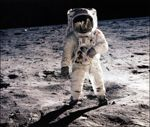
\includegraphics[width=0.8\linewidth]{4x7-triangles-semblables/ex1.pdf}
\end{figure}

Calculer les angles a,b et c. \columnbreak

\Pointilles[8]
\end{multicols}

\subsection*{Ex 2 : Démontrer}

\begin{multicols}{2}
\begin{figure}[H]
  \centering
  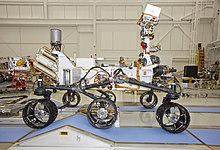
\includegraphics[width=0.6\linewidth]{4x7-triangles-semblables/ex3.pdf}
\end{figure}

Les triangles ABC et DEF sont-ils semblables ?

\columnbreak

\Pointilles[8]
\end{multicols}

\subsection*{Ex 3 : Calculer}

Les tableaux sont proportionnels. 

\begin{multicols}{2}
\begin{center}
  \begin{tabular}{|c|c|c|}
    \hline
    8 & 282 & 801 \\  \hline
    38 & $x$ & $y$\\  \hline
  \end{tabular}
\end{center}

\begin{enumerate}
  \item[1a.] Donner le coefficient de proportionnalité.
  \item[1b.] Calculer $x$ et $y$.
  \end{enumerate}

\begin{center}
  \begin{tabular}{|c|c|c|}
    \hline
    81 & 295 & t \\  \hline
    21 & $z$ & 55\\  \hline
  \end{tabular}
\end{center}

\begin{enumerate}
  \item[2a.] Donner le coefficient de proportionnalité.
  \item[2b.] Calculer $z$ et $t$.
  \end{enumerate}
\end{multicols}

\Pointilles[8]

\newpage

\begin{multicols}{2}
\subsection*{Ex 4 : Triangles semblables}

Les triangles AZE et RTY sont semblables.\\ Calculer $u$ et $v$. 

\begin{figure}[H]
  \centering
  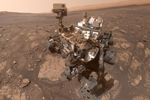
\includegraphics[width=0.7\linewidth]{4x7-triangles-semblables/ex5.pdf}
\end{figure}
\end{multicols} 

\Pointilles[5]

\subsection*{Pb1 : Pendentif} 

\begin{multicols}{2}
Les triangles ABC et SFH de ce pendentifs sont deux triangles isocèles semblables. \\ 

On a : SH = 3,8cm, BC = 3,5cm et FH = 5,5cm. \\ 
Calculer la longueur AB.

\begin{figure}[H]
  \centering
  \includegraphics[width=0.4\linewidth]{4x7-triangles-semblables/pb1.pdf}
\end{figure}

\end{multicols} 

\subsection*{Pb2 : Geyzer}

\begin{figure}[H]
  \centering
  \includegraphics[width=0.4\linewidth]{4x7-triangles-semblables/pb2.pdf}
\end{figure}

Pour estimer la hauteur d'un geyzer [GS], un explorateur [AB] le regarde dans un miroir posé sur le sol en V dans lequel il réussit à voir le sommet G. \\

Calculer la hauteur de ce geyzer.

\subsection*{Pb3 : Problème théorique}

\begin{multicols}{2}

  Les triangles ABC et ACD sont semblables. \\

  Calculer la longueur AB. 

\begin{figure}[H]
  \centering
  \includegraphics[width=0.7\linewidth]{4x7-triangles-semblables/pb3.pdf}
\end{figure}

\end{multicols} 

\end{document}
